\section{Resultados e Discussão}

Simular Gases de Coulomb é especialmente interessante quando não há modelos de matrizes conhecidos, disponíveis ou simples para o $\Hf$ tomado. Podemos, com a simulação de tais gases, calcular a média da função densidade das partículas, ou autovalores, sem ter que diretamente lidar com as matrizes correspondentes. Alternativamente, quando há modelos disponíveis na teoria de RMT, as matrizes poderiam ser diretamente amostradas e a função dos autovalores calculada da diagonalização das mesmas. Tratemos de um caso onde ambas as abordagens são possíveis.

A família de ensembles gaussianos são modelos que mostramos ser bem representados como matrizes na Seção \ref{Section: Ensembles Gaussianos}. Retorne os resultados da Seção \ref{Section: Potencias}. Tomar a medida dos ensembles gaussianos é o equivalente, na simulação de gases descrita, a tomar 
\begin{equation}
d = 1; \ \  n = 2; \ \ \V(x)=\frac{|x|^2}{2}; \ \ W(x) = g(x) = \log{|x|}; \ \ \beta_N = \beta N^2; \ \ \beta = 1,2,4.
\label{Equation: Parametros Gaussian}
\end{equation}
O resultado da simulação para a Configuração \eqref{Equation: Parametros Gaussian} é apresentado na Figura \ref{Figura: Gaussian} para os três modelos ($\beta = 1,2,4$). Na coluna da esquerda, contrasta-se os resultados para $N=10$ da densidade gerada por ambas a simulação de gases e a amostragem direta de matrizes do ensemble. Na coluna central, representa-se a comparação da medida da simulação com o Semi-Círculo de Wigner, configuração de equilíbrio para os três modelos quando $N$ é grande o suficiente. Note que os valores foram escalados por $\sqrt{2 \beta}$ para apresentarem mesmo suporte. Finalmente, na coluna da direita apresentamos a distribuição do maior autovalor $\lambda_{max}$. Um resultado importante enuncia que existem $z_{N}^{(\beta)}$ e $s_N^{(\beta)}$ tais que $$\lim_{N \to \infty} \mathbb{P}_{\beta,N,V} \left( \frac{\lambda_{max} - z_{N}^{(\beta)}}{s_N^{(\beta)}} \leq x \right) = F_{\beta}(x),$$ onde $F_{\beta}(x)$ é a densidade acumulada de Tracy-Widow. \cite{Tracy} 

Observa-se que os dois modelos à esquerda, amostragem direta e simulação de gases, concordam bem na estimativa da medida para o $N$ usado. No centro, é possível notar que a medida de equilíbrio esperada, o Semi-Círculo de Wigner, é aproximada rapidamente pelo aumento de partículas no sistema. A distribuição do autovalor máximo é mais delicada; contudo, ainda que com $N$ finito, podemos ver boa correspondência com o resultado esperado pela Tracy-Widow, piorando com a diminuição da temperatura.
\begin{figure}[ht!]
	\centering
	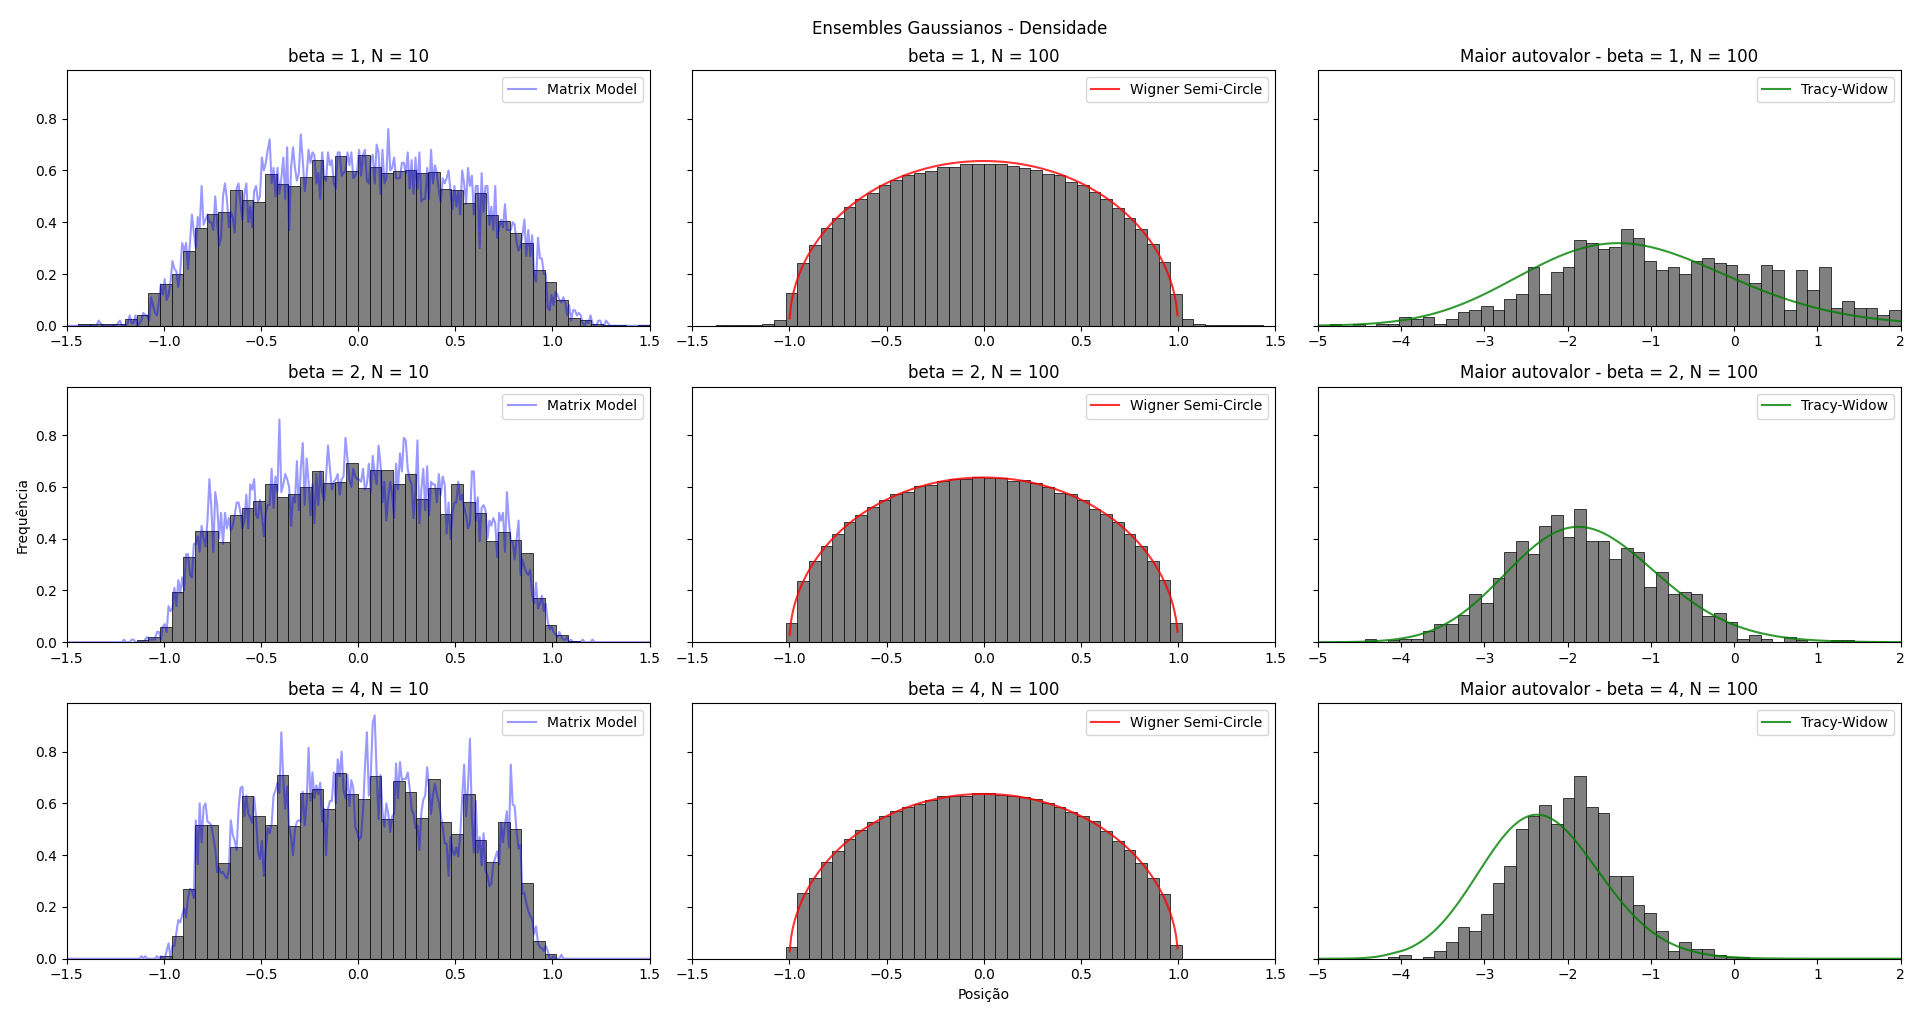
\includegraphics[width=\textwidth]{Assets/validationGaussianTracy.png}
	\caption{Densidade para ensembles gaussianos, \eqref{Equation: Parametros Gaussian}. Tomou-se $\Delta \tilde{t} = 0.1$ e $nsteps = 5\cdot10^6$ passos, registrando a cada $100$ iterações a partir de $nsteps/5$. À esquerda da figura, em azul, a densidade da amostragem de $4\cdot10^3$ matrizes do ensemble. No centro, o Semi-Círculo de Wigner, medida de equilíbrio. Na direita, apresenta-se a densidade de $\lambda_{max}$ normalizado e sua medida esperada.}
	\label{Figura: Gaussian}
\end{figure}

Podemos retomar também as descrições dos potenciais mônico, na Equação \eqref{Equação: Mônico}, e os dois regimes do potencial quártico, Caso \eqref{Equação: Quartico +} e Caso \eqref{Equação: Quartico -}. Respectivamente, estes modelos equivalem a tomar na simulação os parâmetros
\begin{equation}
	d = 1; \ \  n = 2; \ \ \V(x)= t |x|^{2m}; \ \ W(x) = g(x) = \log{|x|}; \ \ \beta_N = \beta N^2; \ \ \beta = 2.
	\label{Equation: Parametros Monico}
\end{equation}
\begin{equation}
	d = 1; \ \  n = 2; \ \ \V(x)=\frac{|x|^4}{4} + t \frac{|x|^2}{2}; \ \ W(x) = g(x) = \log{|x|}; \ \ \beta_N = \beta N^2; \ \ \beta = 2.
	\label{Equation: Parametros Quartico}
\end{equation}
O caso mônico se reduz ao gaussiano se $m=1$. Os resultados para ambos os potenciais estão explicitados na Figura \ref{Figura: Quartic Monic} para alguns parâmetros interessantes de $t$ e $m$.
\begin{figure}[ht!]
	\centering
	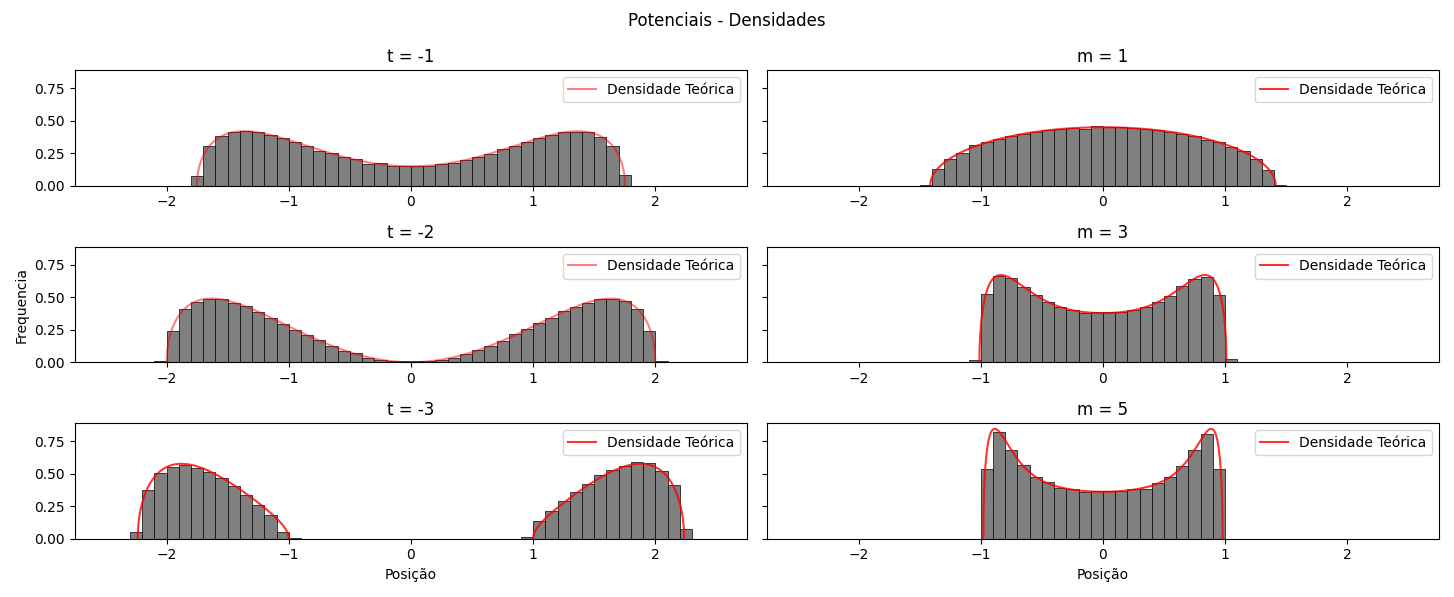
\includegraphics[width=\textwidth]{Assets/validationQuarticMonic-alt.png}
	\caption{Potencial Quártico \eqref{Equation: Parametros Quartico} e Mônico \eqref{Equation: Parametros Monico}, respectivamente à esquerda e direita. Tomou-se $\Delta \tilde{t} = 0.1$, $N=100$, e $nsteps = 5\cdot10^6$ passos. Registra-se a cada $1000$ iterações a partir de $nsteps/5$. No Quártico, simula-se $t=-1,-2,-3$. No Mônico fixa-se $t=1$ e simula-se $m=1,3,5$.}
	\label{Figura: Quartic Monic}
\end{figure}

Novamente as medidas experimentais parecem convergir para a medida teórica enunciada em todas as configurações testadas. Contudo, isso é discutido, com exceção do Mônico, por Chafa\"{i} e Ferré \cite{Chafa2018}. Em luz da situação recentemente explorada por Balogh \textit{et al.} \cite{balogh2016orthogonal} consideremos a Configuração \eqref{Equation: Complex} complexa. Para esta, representamos as medidas simuladas para alguns valores de interesse de $t, a$ na Figura \ref{Figura: Complex},
\begin{equation}
	d = 2; \  n = 2; \  \V(z)=|z|^{2a} - \Re{t z^a};  \ W(x) = g(x) = \log{|x|};  \ \beta_N = \beta N^2;  \ \beta = 2.
	\label{Equation: Complex}
\end{equation}

\begin{figure}[ht]
	\centering
	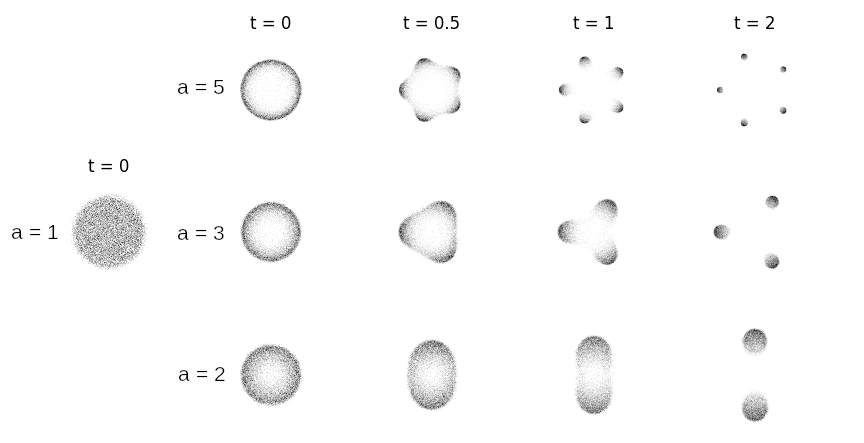
\includegraphics[width=\textwidth]{Assets/complexPotential.png}
	\caption{Medidas referentes à configuração \eqref{Equation: Complex}. Tomou-se $\Delta \tilde{t} = 0.5$ e $nsteps = 2\cdot10^6$ passos, registrando a cada $500$ iterações a partir de $nsteps/5$.}
	\label{Figura: Complex}
\end{figure}

É previsto para esse modelo uma transição de regime - uma separação da medida de equilíbrio - para $t_c \approx \sqrt{\frac{1}{a}}$, o que pode ser observado na Figura \ref{Figura: Complex} com algum detalhe. Outros fatores que corroboram o bom comportamento do modelo são que a medida é uniforme no disco quando $(a,t) = (1,0)$ e se concentra no bordo quando incrementa-se $a$, fatos também previstos. \cite{balogh2016orthogonal} Esse exemplo demonstra que é possível, sem muito esforço, replicar a medida, e principalmente o suporte, para potenciais mais complexos estudados em publicações recentes no tema e pode ser estendido para outros estudos, como para o potencial discutido por Bleher e Silva \cite{Silva}. 

No Capítulo \ref{Capitulo: Intro} apresentamos os ensembles gaussianos como os únicos ensembles invariantes de entradas independentes. Gerar matrizes de outros modelos invariantes dependeria de se saber construir matrizes de entradas não trivialmente correlacionadas. Por outro lado, se sabemos valer a decomposição espectral $\matriz{M} = \matriz{U} \matriz{\Lambda} \matriz{U}^{-1}$, resta que saibamos simular os autovalores para reconstruir as matrizes. Os autovetores podem ser amostrados uniformemente do espaço adequado nos ensembles invariantes. Agora, com a simulação de Gases de Coulomb, apresenta-se uma alternativa para tais distribuições de autovalores. Esse fato, por permitir a reconstrução destas matrizes, possibilita a exploração de múltiplas construções matemáticas que dependem de sua adequada amostragem.

%já que, se tratando de ensembles invariantes, podemos simular matriz $\matriz{U}$ de autovetores distribuídos uniformemente no espaço correspondente. Isso pois sabemos do teorema espectral que, para as matrizes tomadas, vale a decomposição $\matriz{M} = \matriz{U} \matriz{\Lambda} \matriz{U}^{-1}$. Para reconstruir um elemento do ensemble de interesse nos resta replicar a medida de autovalores da matriz $\matriz{\Lambda}$. Isso, de forma interessante, pode ser feito pela simulação descrita de Gases de Coulomb, que replica a medida dos autovalores dos ensemble.

%Outra possibilidade interessante da replicação numérica dessas medidas é que, miniminizada a energia livre $E_{N, V}$, podemos fazer estimativas para constantes da expansão para $\log(Z_{\beta_N})$ proposta em trabalhos recentes, como em \cite{Byun_2023}. Essas estimativas podem dar uma ideia geral do comportamento dessas constantes, de relevante significado físico, para sistemas de interesse.  
